\subsection{GPU Force Calculation Kernel}

In the original GPU kernel implementation, each thread block calculates the forces on the atoms in one patch (patch 1)
due to the atoms in another patch (patch 2). Fig.~\ref{figs:pseudocode} presents the pseudo-code for kernel calculation.
In the outer loop, each thread copies atoms from patch 1 to local registers. In the inner loop. threads in the block collaborate to
load atoms from patch 2 to shared memory. Before and after reading of atoms in patch 2, there are synchronization calls to guarantee
that data is ready to be used before the calculation and is ready to be rewritten after the calculation. During the force
calculation phase, each thread iterates atoms in patch 2 and computes the distance with current atom in patch 1.
If the distance is within cut-off distance, it accumulates the forces for the current atom in patch 1 and finally writes force results
back to GPU global memory. The kernel also calculate a pairlist every 10 time steps used by following time steps to further avoid redundant work. 

\begin{figure}[h]
\centering
\setlength{\abovecaptionskip}{-1pt}
\setlength{\belowcaptionskip}{-2pt}
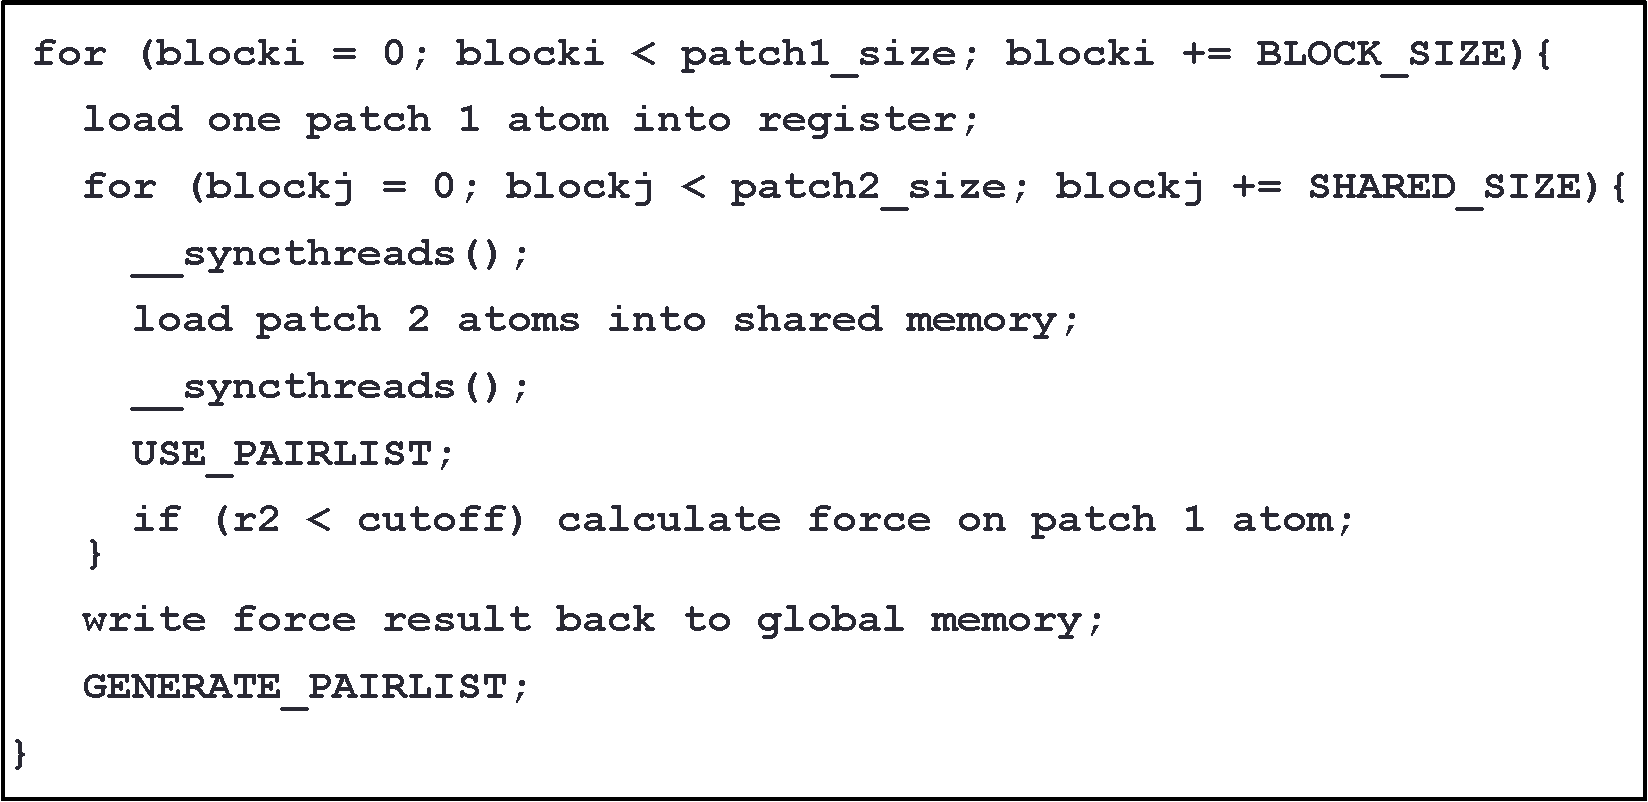
\includegraphics[width=4.0in]{figs/pseudocode-eps-converted-to}
\caption{Pseudocode for GPU kernel force calculation}
\label{figs:pseudocode}
%\vspace{-0.5cm}
\end{figure}

After profiling the performance of the GPU kernel, we acquired the following observations:
(1) force calculation dominates the most GPU time compared to data loads and stores;
(2) there are great control divergence among different threads due to thread synchronization, which means some threads take a really long time
to reach the synchronization where other threads reach it very quickly. However, all threads in the block have to wait for everyone to
reach the synchronization before they can process further. Besides, use of pairlist may aggravate the divergence.
Based on above observations, we proposed several optimization approaches to reduce the control
divergence. They are described in detail in following sections.

\subsection{Optimizations}
\subsubsection{Patch 1 Atoms Tiling}

As indicated in Fig.~\ref{figs:pseudocode}, in each outer loop, for one atom in patch 1, every thread needs to iterate and examine all loaded atoms from patch 2
and call synchronization routines. In order to reduce the synchronization overhead, we first considered tiling of patch 1 atoms,
in which every thread loads mulitple atoms instead of only one atom from patch 1 in each outer loop.
By doing this, total number of outer loops can be reduced. Furthermore, data reuse of patch 2 is improved because now atoms from patch 2 is used to calculate
forces of more atoms from patch 1.

Fig.~\ref{figs:divergence} shows an example of how merging loops can improve the performance. Suppose thread 1 (T1) has 9 units of computation in the first loop and 2 units
of computation in the second loop, whereas thread 2 (T2) has 3 units to do in the first loop and 8 units to do in the second loop. In the first loop T2 needs to wait for
completion of T1 while in the second loop T1 needs to wait for T2. Both threads have to spend long time waiting for each other and total synchronization time is 17.
After merging loops on both T1 and T2, divergence between them is reduced, synchronization call is decreased by 1, and now total synchronization time is 11.

\begin{figure}[h]
\centering
\setlength{\abovecaptionskip}{-1pt}
\setlength{\belowcaptionskip}{-5pt}
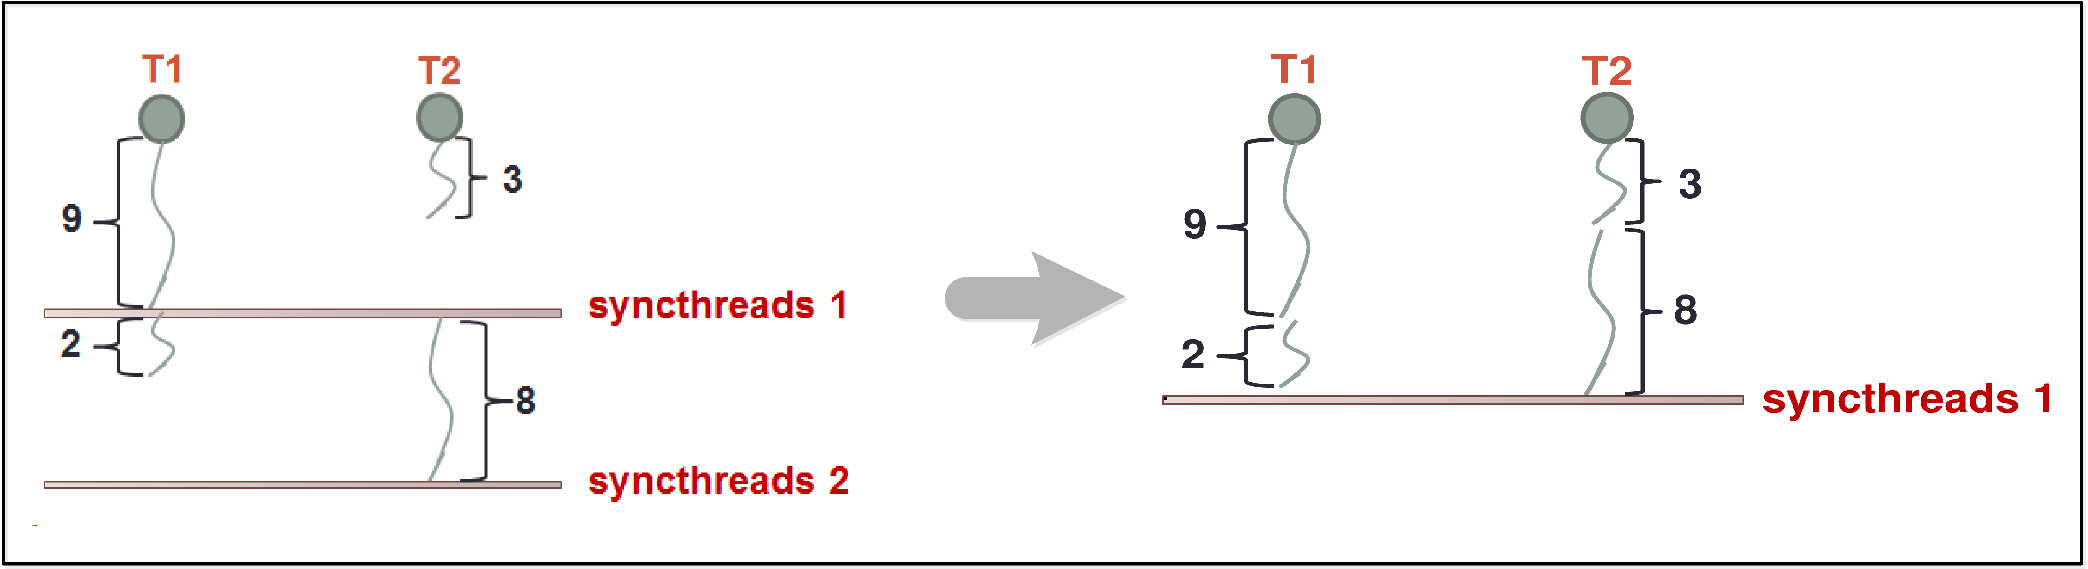
\includegraphics[width=6.0in]{figs/divergence-eps-converted-to}
\caption{Reduce control divergence by merging loops}
\label{figs:divergence}
\vspace{-0.5cm}
\end{figure}

\subsubsection{Patch 2 Atoms Tiling}

After finishing tiling of loading patch 1 atoms, we consider tiling of loading patch 2 atoms to further reduce synchronization calls.
In the original implementation in Fig.~\ref{figs:pseudocode}, for each inner loop, all threads in the thread block collaborate to load SHARED\_SIZE
patch 2 atoms for just one time.
In our optimization, we make all threads load patch 2 atoms multiple times with SHARED\_SIZE in each time. Fig.~\ref{figs:pseudocode-tile} shows
the pseudo-code after tiling is applied. TILE\_WIDTH\_1 and TILE\_WIDTH\_2 are macros to set tile widths for patch 1 and patch 2 correspondingly.

\begin{figure}[h]
\centering
\setlength{\abovecaptionskip}{-1pt}
\setlength{\belowcaptionskip}{-2pt}
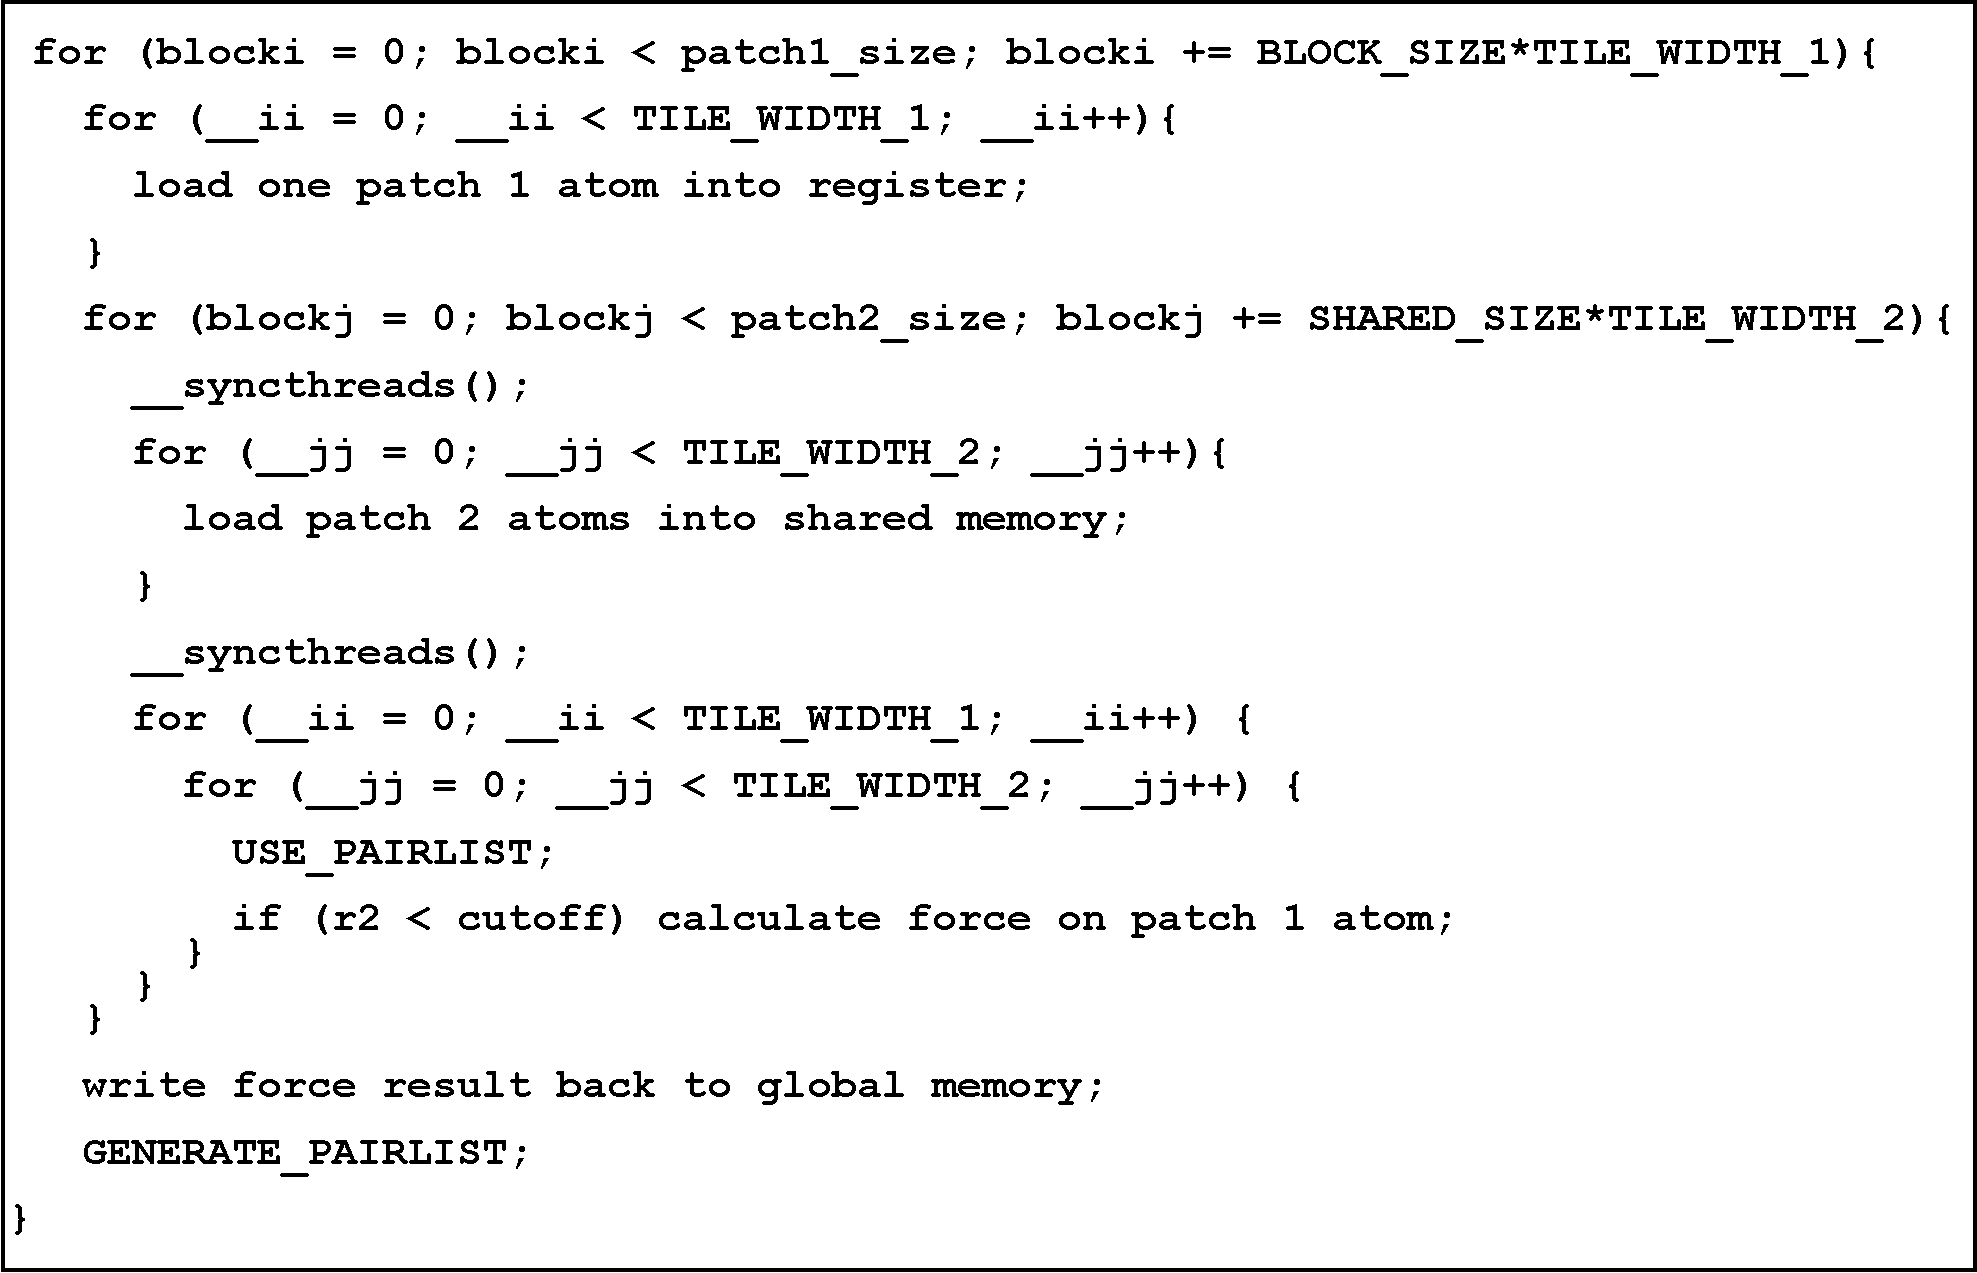
\includegraphics[width=4.0in]{figs/pseudocode-tile-eps-converted-to}
\caption{Pseudocode for GPU kernel force calculation after tiling optimization}
\label{figs:pseudocode-tile}
%\vspace{-0.5cm}
\end{figure}

Fig.~\ref{figs:patch1-count} shows a comparison of computation time among different patch 1 atoms, which is derived by examining a system with 401 atoms in patch 1
and counting how many inner loop needed for each atom. Because there are 401 atoms in total and 128 threads in one thread block, it needs four outer loops to
complete the work. In Fig.~\ref{figs:patch1-count}, region between read dashed lines represents work on atoms assigned to the first
warp and red circles indicate the maximum computation time in current outer loop. The sum results of four read circles is about 920, which indicates
the total work time for the first warp when inner loop is completely tiled and outer loop is not (one synchronization in each outer loop).

Fig.~\ref{figs:thread-count} shows a comparison of computation time among different threads within one thread block, by examining the same system
in Fig.~\ref{figs:patch1-count}. Similarly, region betwen read dashed lines represents work on the first warp. It is shown that the maximum computation time
in this figure is below 800. It inidcates the total work time for the first warp when both inner loop and outer loop are completely tiled (only one synchronization exists). 

\begin{figure}[h]
\centering
\setlength{\abovecaptionskip}{-1pt}
\setlength{\belowcaptionskip}{-2pt}
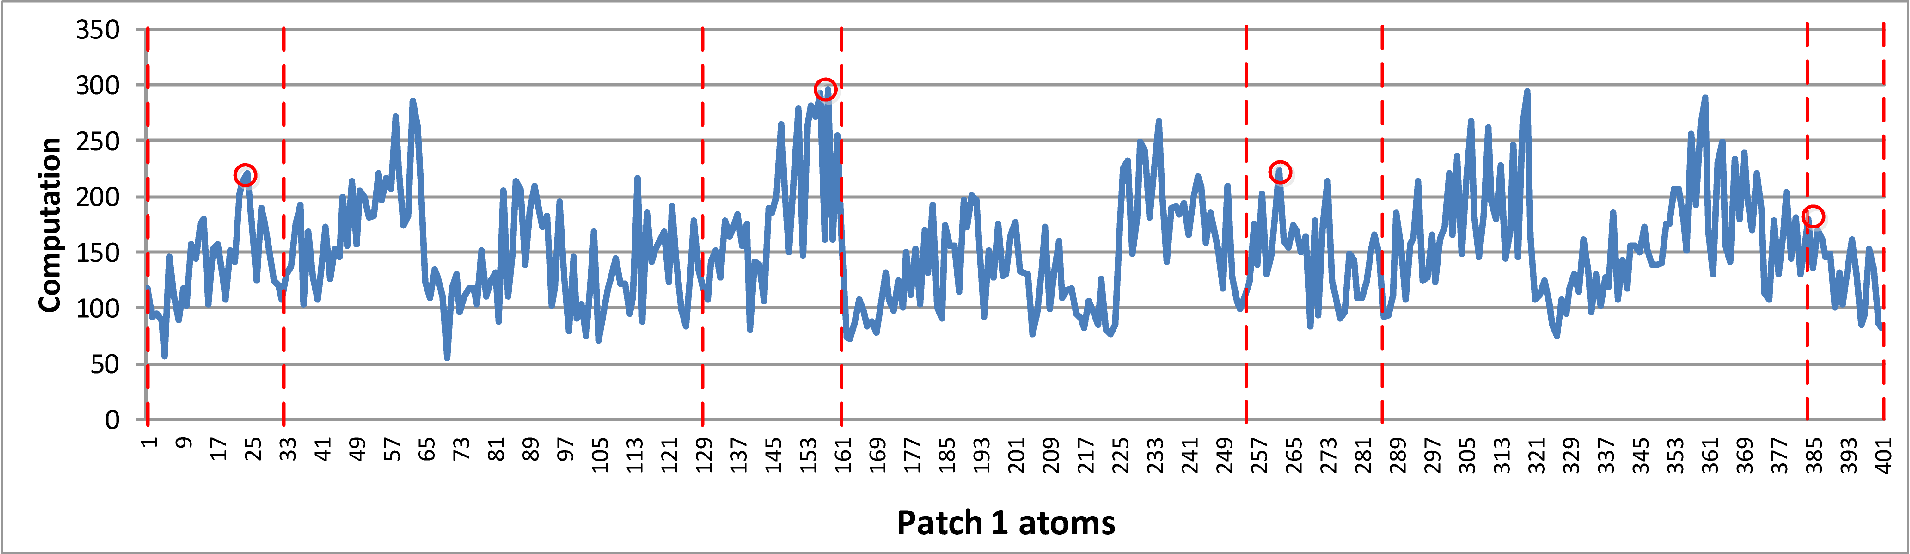
\includegraphics[width=6.0in]{figs/patch1_count-eps-converted-to}
\caption{Computation comparison for different patch 1 atoms}
\label{figs:patch1-count}
\vspace{-0.5cm}
\end{figure}

\begin{figure}[h]
\centering
\setlength{\abovecaptionskip}{-1pt}
\setlength{\belowcaptionskip}{-2pt}
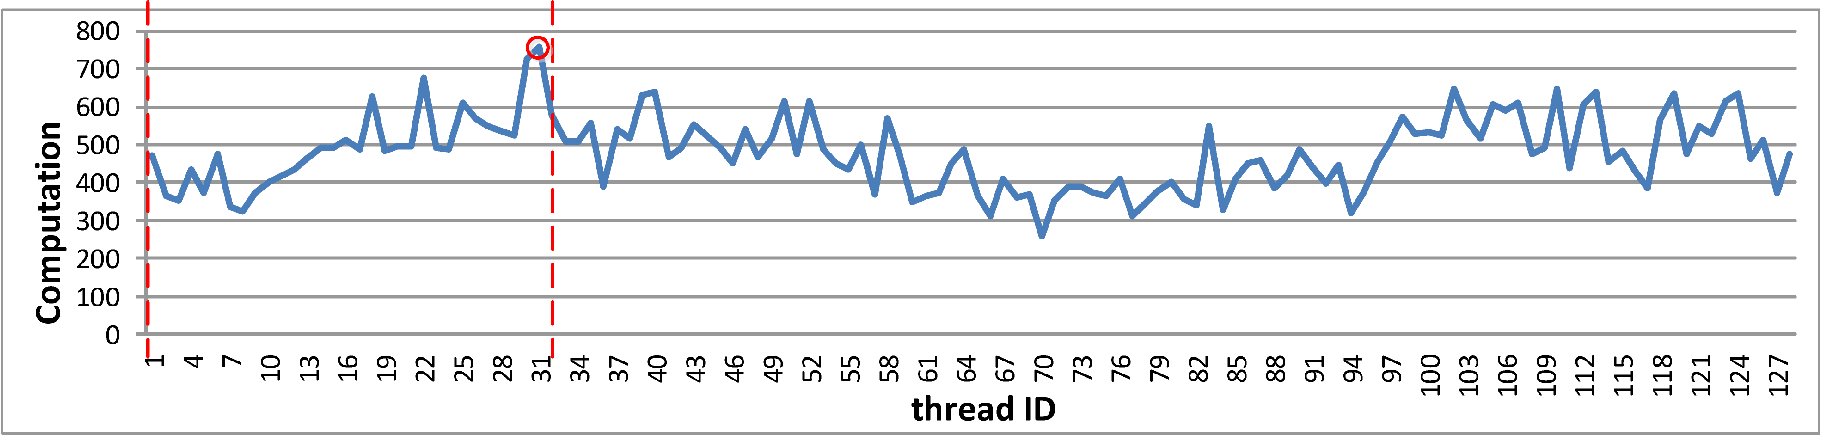
\includegraphics[width=6.0in]{figs/thread_count-eps-converted-to}
\caption{Computation comparison for different threads}
\label{figs:thread-count}
\vspace{-0.3cm}
\end{figure}

\subsubsection{Patch 1 Atoms Sorting}

Inspite of merging loops, we observe that control divergence still exists because there are some threads that always have large work and some threads
that always have small work in each loop. In this case, merging loops would not make a big difference since threads still have to wait for those with
large work to finish. To reduce the control divergence, an effective optimization approach is assigning patch 1 work in a more regular way.
In each time step, we first sort the patch 1 atoms according to their workload, and then pass the sorting result to the next time step to assign the work to threads.
By assigning patch 1 atoms based on sorting instead of randomly, work differences among threads within one warp is not as large as before, and large work
are all assigned to the last warps. The workload on atoms is not changed very little between consecutive time steps, therefore sorting result from the last time step
can be applied to the current time step. 

In our current code, we implement the basic sorting algorithm. This algorithm has the problem that threads which are assigned the least work in the beginning will always
get less work, and same for threads which get the most work. A better strategy to assign the work should be to sort the first 128 atoms in the ascending order,
and the second 128 atoms in the descending order, and the third 128 atoms in the ascending order, and so on. In this way, threads who get less work in the first
iteration will get more work in the next iteration. Work can be assigned more evenly.
